\documentclass[12pt,a4paper]{report}
\usepackage{titlesec} %these are how we import packages, one helps set up footers and title layout
\usepackage{fancyhdr}

% !TEX TS-program = pdflatex
% !TEX encoding = UTF-8 Unicode
\usepackage[utf8]{inputenc} % set input encoding (not needed with XeLaTeX)
\usepackage{graphicx} % support the \includegraphics command and options

%%% PACKAGES
\usepackage{booktabs} % for much better looking tables
\usepackage{array} % for better arrays (eg matrices) in maths
\usepackage{paralist} % very flexible & customisable lists (eg. enumerate/itemize, etc.)
\usepackage{booktabs}
\usepackage{verbatim} % adds environment for commenting out blocks of text & for better verbatim
\usepackage{subfig} % make it possible to include more than one captioned figure/table in a single float
\usepackage[square,sort]{natbib}
\usepackage{tikz}
\usetikzlibrary{er,positioning}
\usepackage{longtable}
\usepackage{rotating}
\usepackage{pdflscape}
\usepackage[toc,page]{appendix}
% These packages are all incorporated in the memoir class to one degree or another...
\usepackage{amsmath}
\usepackage{supertabular}
\usepackage{pdfpages}
\usepackage{amsthm}
\theoremstyle{definition}
\newtheorem{definition}{Definition}[chapter]

%header and footer settings
\pagestyle{fancyplain}
\fancyhf{}
\renewcommand{\headrulewidth}{0.5pt}
\renewcommand{\footrulewidth}{0.5pt}
\setlength{\headheight}{15pt}
\fancyhead[L]{Marcin Szczot - 40180425}
\fancyhead[R]{ SOC10101 Honours Project}
\fancyfoot[L]{}
\fancyfoot[C]{\thepage}

%set better section layout
\makeatletter
\renewcommand\subsection{\@startsection {subsection}{1}{2mm} % name, level, indent
                               {3pt plus 2pt minus 1pt} % before skip
                               {3pt plus 0pt} % after skip
                               {\normalfont\bfseries}}
\renewcommand\subsubsection{\@startsection {subsubsection}{2}{4mm} % name, level, indent
                               {3pt plus 2pt minus 1pt} % before skip
                               {3pt plus 0pt} % after skip
                               {\normalfont\bfseries}}
\makeatother
\makeatletter
\renewcommand\section{\@startsection {section}{1}{0mm} % name, level, indent
                               {4pt plus 2pt minus 1pt} % before skip
                               {4pt plus 0pt} % after skip
                               {\bfseries}}
\makeatother

\graphicspath{{./img/}}

%this starts the document
\begin{document}

\begin{titlepage}
	\centering
	{\scshape\LARGE Edinburgh Napier University \par}
	\vspace{1cm}
	{\scshape\Large Week 9 Report\par}
	\vspace{1.5cm}
	{\huge\bfseries Computing abstract argumentation semantics\par}
	\vspace{2cm}
	{\Large Marcin Szczot\par}
	{\Large 40180425\par}
	\vfill
	supervised by\par
	Dr. S. \textsc{Wells}

	\vfill

% Bottom of the page
	{\large \today\par}
\end{titlepage}

\tableofcontents % is generated for you
\newpage

\listoftables
%generated in same way as figures
\newpage

\listoffigures
%you may have captions such as equations, listings etc they should all appear as required
%these are done for you as long as you use \begin{figure}[placement settings] .. bla bla ... \end{figure}
\newpage


%-------------------------------------------------------------------------------
% Variables
%-------------------------------------------------------------------------------
\newcommand{\software}{\textit{Alias}}
%-------------------------------------------------------------------------------
% End of Variables 
%-------------------------------------------------------------------------------

%-------------------------------------------------------------------------------
% Main content 
%-------------------------------------------------------------------------------
\chapter{Introduction}

-------------------------------------------------------------------------------\\
\textbf{Points to discuss:}
\begin{enumerate}
	\item{Overall aim of the project}
	\item{Main goals for each stage of the project}
	\item{Goals for the software}
\end{enumerate}
-------------------------------------------------------------------------------\\

The aim of this project is to implement high performance, scalable library for computing abstract argumentation semantics (complete, preffered, stable, grounded, semi-stable and stage semantics) for given argumentation framework. Furthermore, it should have the ability to compute if the given argument from the given argumentation framework is credulously or skeptically inferred for given semantics.
This project can be divided into four separate stages: research, design, development and evaluation. Although the stages proposed can be performed in the sequence, work on this project will be performed in the iterative way. In the work plan for the project, 3 iterations of desing, development and testing have been identified. Additionally, further research might be required in the later stages. Each stage of the project have overall goals that will neeed to be achieved. 

Research and review stage is the vital part of the project. This will allow to build a better understanding of the problem domain and investigate existing solutions. Following goals can be identified for this stage:
\begin{enumerate}
	\item{Research concept of argumentation framework and abstract argumentation semantics}
	\item{Research and review existing algorithms for solving the problem}
	\item{Review solvers submitted to ICCMA 2017}
	\item{Perform technology review}
\end{enumerate}

Once enough research will be performed, the project can proceed to next stages. The knowledge gathered will be used to define the requirements and propose appropriate solution. The design, development and testing stages will be performed in an iterative way. Goals for those stages include:
\begin{enumerate}
	\item{Perform Requirements Analysis}
	\item{Define Test Plan}
	\item{Based on the requirements analysis design appropriate solution} 
	\item{Implement the proposed solution}
	\item{Test the solution to verify implemented requirements}
	\item{Perform benchmark testing to evaluate the performance and correctness of the solution}
\end{enumerate}
As mentioned above, 3 iterations of those stages have been initially scheduled. Additionaly, during any of those stages further research might be required. 
\newline
The outcome of the project will be the developed library for computing abstract argumentation framework. Furthermore, depending on the evaluation process, the library will be used to develop a solver for abstract argumentation framework to be submitted to International Competition on Computational Models of Argumentation \cite{ICCMA}. Hence there are number of requirements that will have to be included in the implementation.

\chapter{Background}
Argumentation framework is central to the theory of abstract argumentation \cite{baroni2011introduction}. The argumentation framework is defined as a pair of a set of arguments, and a binary relation representing the attack relationship between arguments \cite{dung1995}. 

\theoremstyle{definition}
\begin{definition}{Argumentation Framework}
\label{AFdef}\\
An argumentation framework is a pair \textit{AF} = $<$\textit{AR, attacks}$>$ in which \textit{AR} is a set of finite arguments, and \textit{attacks} is a binary relation on \textit{AR}, hence \textit{attacks} $\subseteq$ \textit{AR} $\times$ \textit{AR}
\end{definition}

In definition \ref{AFdef}, \textit{attacks} represents set of pairs of arguments (\textit{a, b}), where (\textit{a, b}) $\in$ \textit{attacks}. Each pair of arguments in \textit{attacks} represents two arguments being in conflict. Hence, the arguments \textit{a} and \textit{b} are in conflict and the meaning of of \textit{attacks(a, b)} is that \textit{a} represents an attack agains \textit{b} \cite{dung1995}.

Dung in his paper \cite{dung1995} has also defined futher notions for argumentation framework, which are as follow:
\begin{enumerate}
	\item{An argument \textit{a} $\in$ \textit{AR} is acceptable with }
\end{enumerate}

The argumentation framework can be represented as directed graph where the nodes represent abstract arguments and edges the attack relation. This can be seen in figure \ref{fig:argumentationFrameworkFigure}, where argument a attacks argument b, which in turn attacks argument c. C is also attacked by argument d.

\begin{figure}[h]
	\centering
	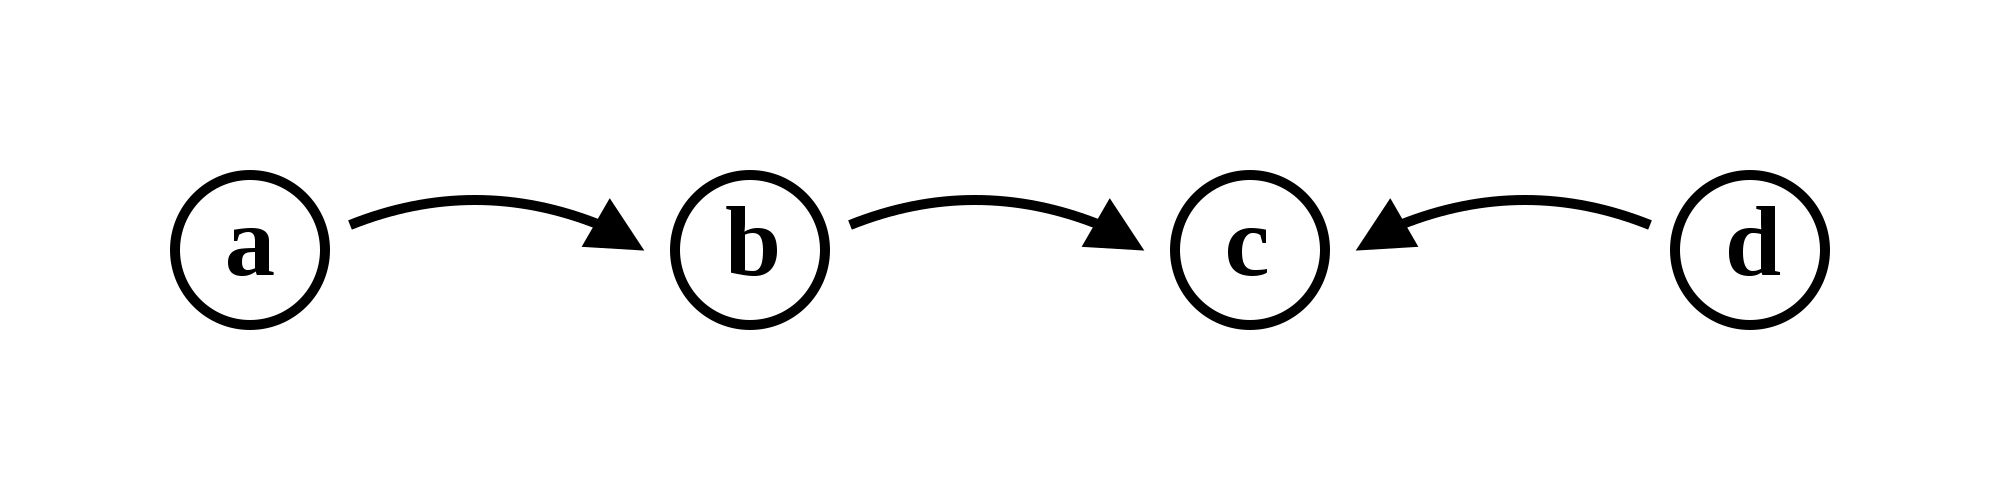
\includegraphics[width=\textwidth,keepaspectratio=true]{argumentationFramework.png}
	\caption{Representation fo argumentation framework, from \cite{argumentationFrameworkExample}}
	\label{fig:argumentationFrameworkFigure}
\end{figure}

 

\chapter{Plan of Work}

-------------------------------------------------------------------------------\\
\textbf{Points to discuss:}
\begin{enumerate}
	\item{\textit{Schedule for the project}}
	\item{\textit{Design, development and testing cycles}}
\end{enumerate}
-------------------------------------------------------------------------------\\


\chapter{Project Evaluation}

-------------------------------------------------------------------------------\\
\textbf{Points to discuss}
\begin{enumerate}
	\item{Define clear way of evaluating the project}
	\item{Describe benchmark testing}
	\item{Define analysis of benchmark testing results}
\end{enumerate}
-------------------------------------------------------------------------------\\

The project will be evaluated based on the benchmark testing. Benchmark tests will be performed after each developement cycle and will be used to evaluate the performance and correctness of the software based on the results from the solvers submitted for the second edition of International Competition on Computational Models of Argumentation (http://argumentationcompetition.org/). 
The benchamrk tests will include computing semantics from provided argumentation frameworks. It will be split into 7 tracks. Each track will represent different semantic. Following semantics will be used for benchmark testing:
\begin{enumerate}
	\item{Complete Semantics - CO}
	\item{Preferred Semantics - PR}
	\item{Stable Semantics - ST}
	\item{Semi-Stable Semantics - SST}
	\item{Stage Semantics - STG}
	\item{Grounded Semantics - GR}
	\item{Ideal Semantics - ID}
\end{enumerate}

For each track the system will need to solve following reasoning problems, with the exception for Grounded and Ideal semantics where only A and C are applicable:
\begin{enumerate}
	\item{Given an abstract argumentation framework, determine some extension\\SE-$\sigma$: Given F=(A,R) return some set E $\subseteq$ A that is a $\sigma$-extension}
	\item{Given an abstract argumentation framweork, determine all extensions\\EE-$\sigma$: Given F=(A,R) enumerate all sets E $\subseteq$ A that are $\sigma$-extensions}
	\item{Given an abstract argumentation framework and some argument, decide whether the given argument is credulously inferred\\DC-$\sigma$ : Given F=(A,R), a $\in$ A decide whether a is credulously accepted under $\sigma$}
	\item{Given an abstract argumentation framework and some argument, decide whether the given argument is skeptically inferred\\DS-$\sigma$: Given F=(A,R), a $\in$ A decide whether a is skeptically accepted under $\sigma$}
\end{enumerate}

There are 4 different benchmarks that will be used (all of them were used for testing solvers submitted to ICCMA 2017). Each benchmark group consist of a number of abstract argumentation frameworks in formats \textit{apx} and \textit{tgf}. Furthermore, each group of argumentation frameworks are used for a specific tasks. The list of relations between benchmarks and the tasks is below:
\begin{itemize}
	\item{Benchmark A - DS-PR, EE-PR, EE-CO, DS-SST, DC-SST, SE-SST, EE-SST, DS-STG, DC-STG, SE-STG, EE-STG}
	\item{Benchmark B - DS-ST, DC-ST, SE-ST, EE-ST, DC-PR, SE-PR, DC-CO}
	\item{Benchmark C - DS-CO, SE-CO, DC-GR, SE-GR}
	\item{Benchmark D - DC-ID, SE-ID}
\end{itemize}

Prior to running the benchmarking tests following solvers will need to be tested with the available benchmarks to evaluate their performance in the given environment.
\begin{enumerate}
	\item{pyglaf - CO, ST, ID tracks}
	\item{ArgSemSAT - PR track}
	\item{argmat-sat - SST, STG tracks}
	\item{CoQuiAAS v2.0 - GR track}
\end{enumerate}
Those are the winning solvers in the specified tracks. Once the baseline for benchmark testing will be created, the software testing can commence.



%-------------------------------------------------------------------------------
% End of Main content 
%-------------------------------------------------------------------------------

\newpage
\bibliographystyle{apalike}
\bibliography{references}
%example of References. See https://en.wikibooks.org/wiki/LaTeX/Bibliography_Management
%might be good to use a separate document for these so your main work is not one really long text file. 

%you can crate this on a extra tex document just like the title or any other part of the document.
\newpage
\begin{appendices}
\chapter{Initial Project Overview}
\label{appendix:IPO}
\textbf{Initial Project Overview} \\
\textbf{SOC10101 Honours Project (40 Credits)}             \\                                          
\textbf{Title of Project: Computing abstract argumentation semantics }\\

\section{Overview of Project Content and Milestones}
The aim of this project is to implement scalable software for computing semantics (preferred, stable, grounded, etc.) of abstract argumentation from the given argumentation framework. This project will have a number of milestones that will need to be achieved. They include research of the argumentation framework semantics based on Dung’s original notions of complete, grounded, preferred and stable semantics, as well as further proposed notions of semi-stable, stage and ideal semantics. Furthermore, different approaches, such as labelling-based and extension-based approaches along with different algorithms will be reviewed, investigated and evaluated. Additionally, software submitted to the International Competition on Computational Models of Argumentation will be investigated and evaluated based on the approaches used for computing the semantics. Finally, new software will be designed, developed, tested and benchmarked against the solvers from International Competition on Computational Models of Argumentation. The aim will be to produced scalable software for calculating different types of semantics from provided argumentation framework.

\section{The Main Deliverable(s):}
The main deliverables of this project will be the final report, which will include the review of argumentation framework, common algorithms used for calculating abstract argumentation semantics and software to be submitted to ICCMA. The report will also include a review of design, development and testing of the proposed solution. Furthermore, the developed software for computing abstract argumentation semantics will be part of deliverables.

\section{The Target Audience for the Deliverable(s):}
The target audience for projects’ deliverables are the researches working on argumentation in computing.

\section{The Work to be Undertaken:}
This project requires research to be conducted on the argumentation framework and the notion of semantics introduced by Dung and extended by Caminada and others. Existing approaches and algorithms for labelling arguments and calculating the semantics will have to be researched and reviewed. Furthermore, new software for computing the semantics from given argumentation framework will be designed, implemented and tested. Existing solutions will be used for benchmarking the performance and scalability of the developed solution.

\section{Additional Information / Knowledge Required:}
In order to complete the project further knowledge is required in the abstract argumentation frameworks and their semantics. Furthermore, new system for computing the semantics will be developed in Python, hence extensive knowledge will be required for designing and implementing scalable approach for traversing large graphs of argumentation frameworks. 

\section{Information Sources that Provide a Context for the Project:}
The project will be based on the abstract argumentation semantics introduced by Phan Minh Dung in the paper On the acceptability of arguments and its fundamental role in nonmonotonic reasoning, logic programming and n-person games. The semantics were further extended with semi-stable semantics by Martin Caminada in his paper Semi-Stable Semantics, stage semantics by Bart Verheij in Two approaches to dialectical argumentation: admissible sets and argumentation stages and ideal semantics by Phan Minh Dung, Paolo Mancarella and Francesca Toni in Computing ideal sceptical argumentation. Furthermore, the solvers submitted to the International Competition on Computational Models of Argumentations (http://argumentationcompetition.org/) will be used for benchmarking the proposed solution. 

\section{The Importance of the Project:}
Research focus in AI for defeasible reasoning

\section{The Key Challenge(s) to be Overcome:}
Main challenge of this project will be to design and implement universal solution for computing different semantics (complete, preferred, stable, etc.) of abstract arguments in the provided argumentation framework. Furthermore, the solution must be able to scale appropriately and be able to perform calculation on supplied argumentation framework with different structures.


\chapter{Requirement Analysis} 
\label{appendix:requirementAnalysis}
\begin{center}
\label{tab:requirementsAnalysis}
\begin{longtable}{| p{.02\textwidth} | p{.80\textwidth} | p{.18\textwidth} |} 
\hline \multicolumn{1}{|c|}{\textbf{ID}} & \multicolumn{1}{c|}{\textbf{Requirement}} & \multicolumn{1}{c|}{\textbf{MoSCoW}} \\ \hline 
\endfirsthead


\multicolumn{3}{c}%
{{\bfseries \tablename\ \thetable{} -- continued from previous page}} \\
\hline \multicolumn{1}{|c|}{\textbf{ID}} &
\multicolumn{1}{c|}{\textbf{Requirement}} &
\multicolumn{1}{c|}{\textbf{MoSCoW}} \\ \hline 
\endhead

\hline \multicolumn{3}{|r|}{{Continued on next page}} \\ \hline
\endfoot

\hline \hline
\endlastfoot

1  & Should read provided tgf file                                                                                                                           & Must have   \\ \hline
2  & Should parse tgf file                                                                                                                                   & Must have   \\ \hline
3  & Should read provided apx file                                                                                                                           & Should have \\ \hline
4  & Should be able to determine SOME complete extensions from given argumentation framework (SE-CO)                                                         & Should have \\ \hline
5  & Should be able to determine ALL complete extensions from given argumentation framework (EE-CO)                                                          & Should have \\ \hline
6  & Given the argumentation framework and some argument, should decide whether the given argument is credulously inferred in complete extension (DC-CO)     & Should have \\ \hline
7  & Given the argumentation framework and some argument, should decide whether the given argument is sceptically inferred in complete extension (DS-CO)     & Should have \\ \hline
8  & Should be able to determine SOME preferred semantics from given argumentation framework (SE-PR)                                                         & Should have \\ \hline
9  & Should be able to determine ALL preferred extensions from given argumentation framework (EE-PR)                                                         & Should have \\ \hline
10 & Given the argumentation framework and some argument, should decide whether the given argument is credulously inferred in preferred extension (DC-PR)    & Should have \\ \hline
11 & Given the argumentation framework and some argument, should decide whether the given argument is sceptically inferred in preferred extension (DS-PR)    & Should have \\ \hline
12 & Should be able to determine SOME stable extensions from given argumentation framework (SE-ST)                                                           & Should have \\ \hline
13 & Should be able to determine ALL stable extensions from given argumentation framework (EE-ST)                                                            & Should have \\ \hline
14 & Given the argumentation framework and some argument, should decide whether the given argument is credulously inferred in stable extension (DC-ST)       & Should have \\ \hline
15 & Given the argumentation framework and some argument, should decide whether the given argument is sceptically inferred in stable extension (DS-ST)       & Should have \\ \hline
16 & Should be able to determine SOME semi-stable extensions from given argumentation framework (SE-SST)                                                     & Should have \\ \hline
17 & Should be able to determine ALL semi-stable extensions from given argumentation framework (EE-SST)                                                      & Should have \\ \hline
18 & Given the argumentation framework and some argument, should decide whether the given argument is credulously inferred in semi-stable extension (DC-SST) & Should have \\ \hline
19 & Given the argumentation framework and some argument, should decide whether the given argument is sceptically inferred in semi-stable extension (DS-SST) & Should have \\ \hline
20 & Should be able to determine SOME stage extensions from given argumentation framework (SE-STG)                                                           & Should have \\ \hline
21 & Should be able to determine ALL stage extensions from given argumentation framework (EE-STG)                                                            & Should have \\ \hline
22 & Given the argumentation framework and some argument, should decide whether the given argument is credulously inferred in stage extension (DC-STG)       & Should have \\ \hline
23 & Given the argumentation framework and some argument, should decide whether the given argument is sceptically inferred in stage extension (DS-STG)       & Should have \\ \hline
24 & Should be able to determine SOME grounded extensions from given argumentation framework (SE-GR)                                                         & Should have \\ \hline
25 & Should be able to determine ALL grounded extensions from given argumentation framework (EE-GR)                                                          & Should have \\ \hline
26 & Should be able to determine SOME ideal extensions from given argumentation framework (SE-ID)                                                            & Should have \\ \hline
27 & Should be able to determine ALL ideal extensions from given argumentation framework (SE-ID)                                                             & Should have \\ \hline
28 & Should output the result of the computation to command line                                                                                             & Must have   \\ \hline
29 & Should take file format as a command line argument, i.e. -fo {[}file format{]}                                                                          & Must have   \\ \hline
30 & Should take type of task as a command line argument, i.e. -p {[}EE-CO{]}                                                                                & Must have   \\ \hline
31 & Should take file as a command line argument, i.e. -f {[}./argumentationFramework.apx{]}                                                                 & Must have   \\ \hline 
\end{longtable}
\end{center}

\chapter{Project Schedule}
\label{appendix:projectSchedule}
\begin{figure}[h]
	\centering
	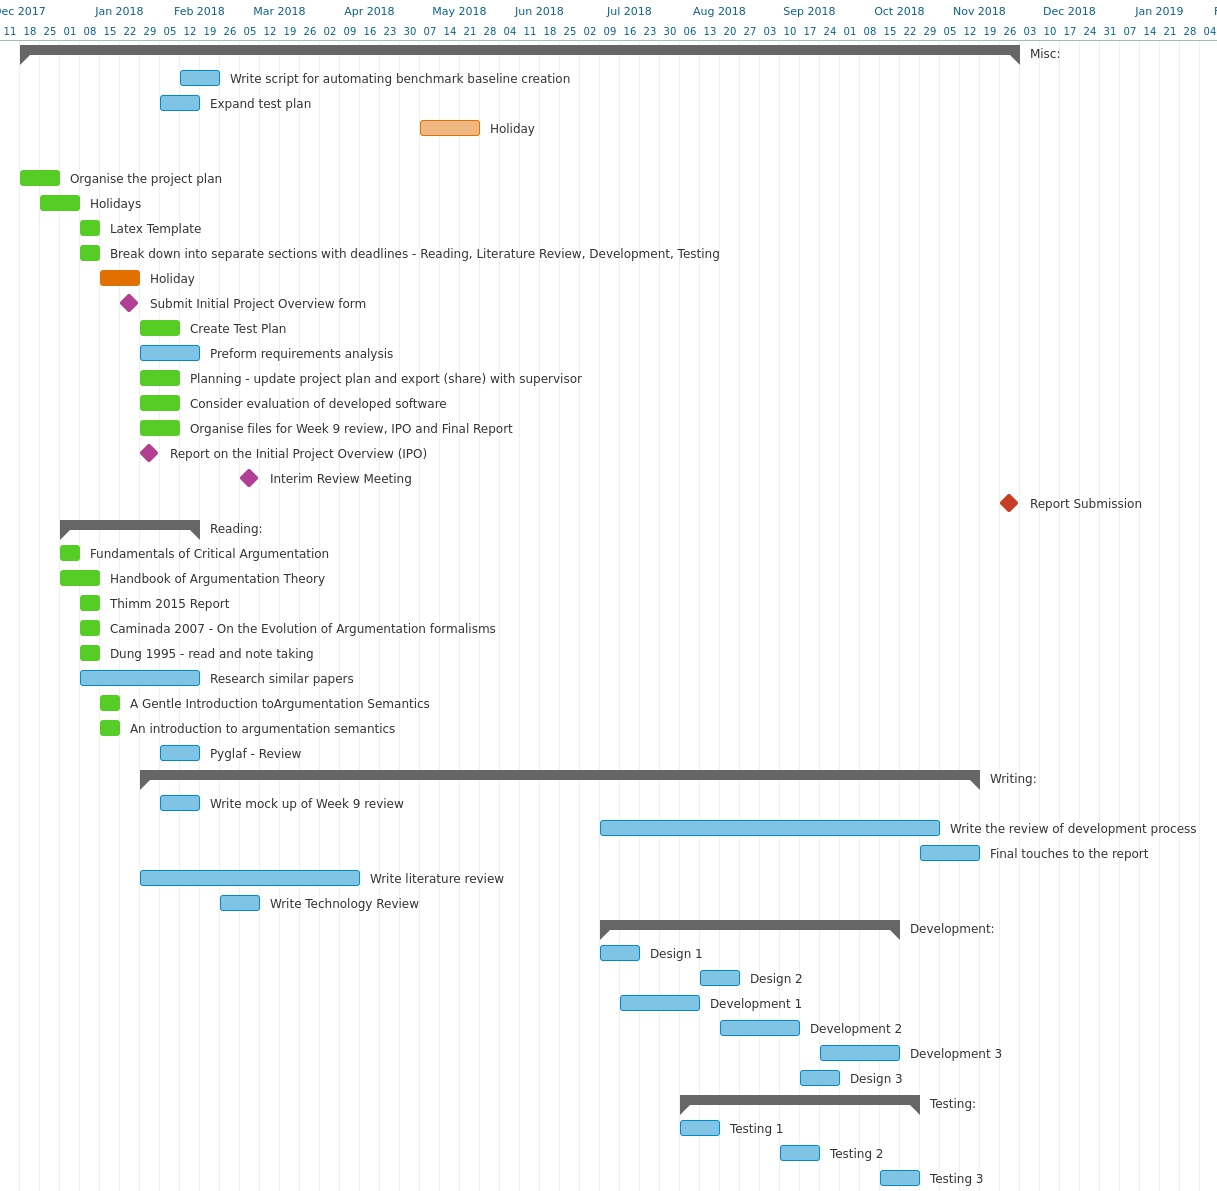
\includegraphics[width=\textwidth]{gantt1}
	\caption{Project Schedule}
	\label{fig:projectSchedule}
\end{figure}

\chapter{Meetings diaries}
\label{appendix:diaries}
\newpage
\includepdf{./diaries/20180116.pdf}
\includepdf{./diaries/20180123.pdf}
\includepdf{./diaries/20180130.pdf}
\includepdf{./diaries/20180206.pdf}
\includepdf{./diaries/20180213.pdf}
\includepdf{./diaries/20180220.pdf}
\includepdf{./diaries/20181008.pdf}

\chapter{ICCMA 2017 Submissions}
\label{appendix:ICCMASubmissions}
\begin{center}
\begin{longtable}{| p{.2\textwidth} | p{.8\textwidth} |}
\caption{ICCMA 2017 Submissions}
\label{table:ICCMA2017Submissions}\\

\hline \multicolumn{1}{|c|}{\textbf{Solver}} & \multicolumn{1}{c|}{\textbf{Author}}\\ \hline 
\endfirsthead


\multicolumn{2}{c}%
{{\bfseries \tablename\ \thetable{} -- continued from previous page}} \\
\hline \multicolumn{1}{|c|}{\textbf{Solver}} &
\multicolumn{1}{c|}{\textbf{Author}} \\ \hline 
\endhead

\hline \multicolumn{2}{|r|}{{Continued on next page}} \\ \hline
\endfoot

\hline \hline
\endlastfoot

argmat-clpb   & Fuan Pu (Tsinghua University, China), Guiming Luo (Tsinghua University, China), Yucheng Chen (Tsinghua University, China).                  \\ \midrule
argmat-dvisat & Fuan Pu (Tsinghua University, China), Guiming Luo (Tsinghua University, China), Ya Hang (Tsinghua University, China).                    \\ \hline
argmat-mpg & Fuan Pu (Tsinghua University, China), Guiming Luo (Tsinghua University, China), Ya Hang (Tsinghua University, China).                    \\ \hline
argmat-sat & Fuan Pu (Tsinghua University, China), Guiming Luo (Tsinghua University, China), Ya Hang (Tsinghua University, China).                    \\ \hline
ArgSemSAT  & Federico Cerutti (Cardiff University, UK), Mauro Vallati (University of Huddersfield, UK), Massimiliano Giacomin (University of Brescia, Italy), Tobia Zanetti (University of Brescia, Italy). \\ \hline
ArgTools   & Samer Nofal (German Jordanian University, Jordan), Katie Atkinson (University of Liverpool, UK), Paul E. Dunne (University of Liverpool, UK).              \\ \hline
ASPrMin    & Wolfgang Faber (University of Huddersfield, UK), Mauro Vallati (University of Huddersfield, UK), Federico Cerutti (Cardiff University, UK), Massimiliano Giacomin (University of Brescia, Italy). \\ \hline
cegartix   & Wolfgang Dvořák (TU Wien, Austria), Matti Järvisalo (University of Helsinki, Finland), Johannes P. Wallner (TU Wien, Austria).                 \\ \hline
Chimærarg  & Federico Cerutti (Cardiff University, UK), Mauro Vallati (University of Huddersfield, UK), Massimiliano Giacomin (University of Brescia, Italy).              \\ \hline
ConArg  & Stefano Bistarelli (Università di Perugia, Italy), Fabio Rossi (Università di Perugia, Italy), Francesco Santini (Università di Perugia, Italy).              \\ \hline
CoQuiAAS   & Jean-Marie Lagniez (Univ. Artois, France), Emmanuel Lonca (Univ. Artois, France), Jean-Guy Mailly (Univ. Paris Descartes, France).                \\ \hline
EqArgSolver   & Odinaldo Rodrigues (King's College London, UK).                                       \\ \hline
gg-sts  & Tomi Jahunen (Aalto University, Finland), Shahab Tasharrofi (Aalto University, Finland).                            \\ \hline
goDIAMOND  & Stefan Ellmauthaler (Leipzig University, Germany), Hannes Strass (Leipzig University, Germany).                           \\ \hline
heureka    & Nils Geilen (Universität Koblenz-Landau, Germany), Matthias Thimm (Universität Koblenz-Landau, Germany).                        \\ \hline
pyglaf  & Mario Alviano (University of Calabria, Italy).                                       
\end{longtable}
\end{center}


\chapter{Argumentation Framework Graph}
\label{appendix:aficcma}
\begin{figure}
	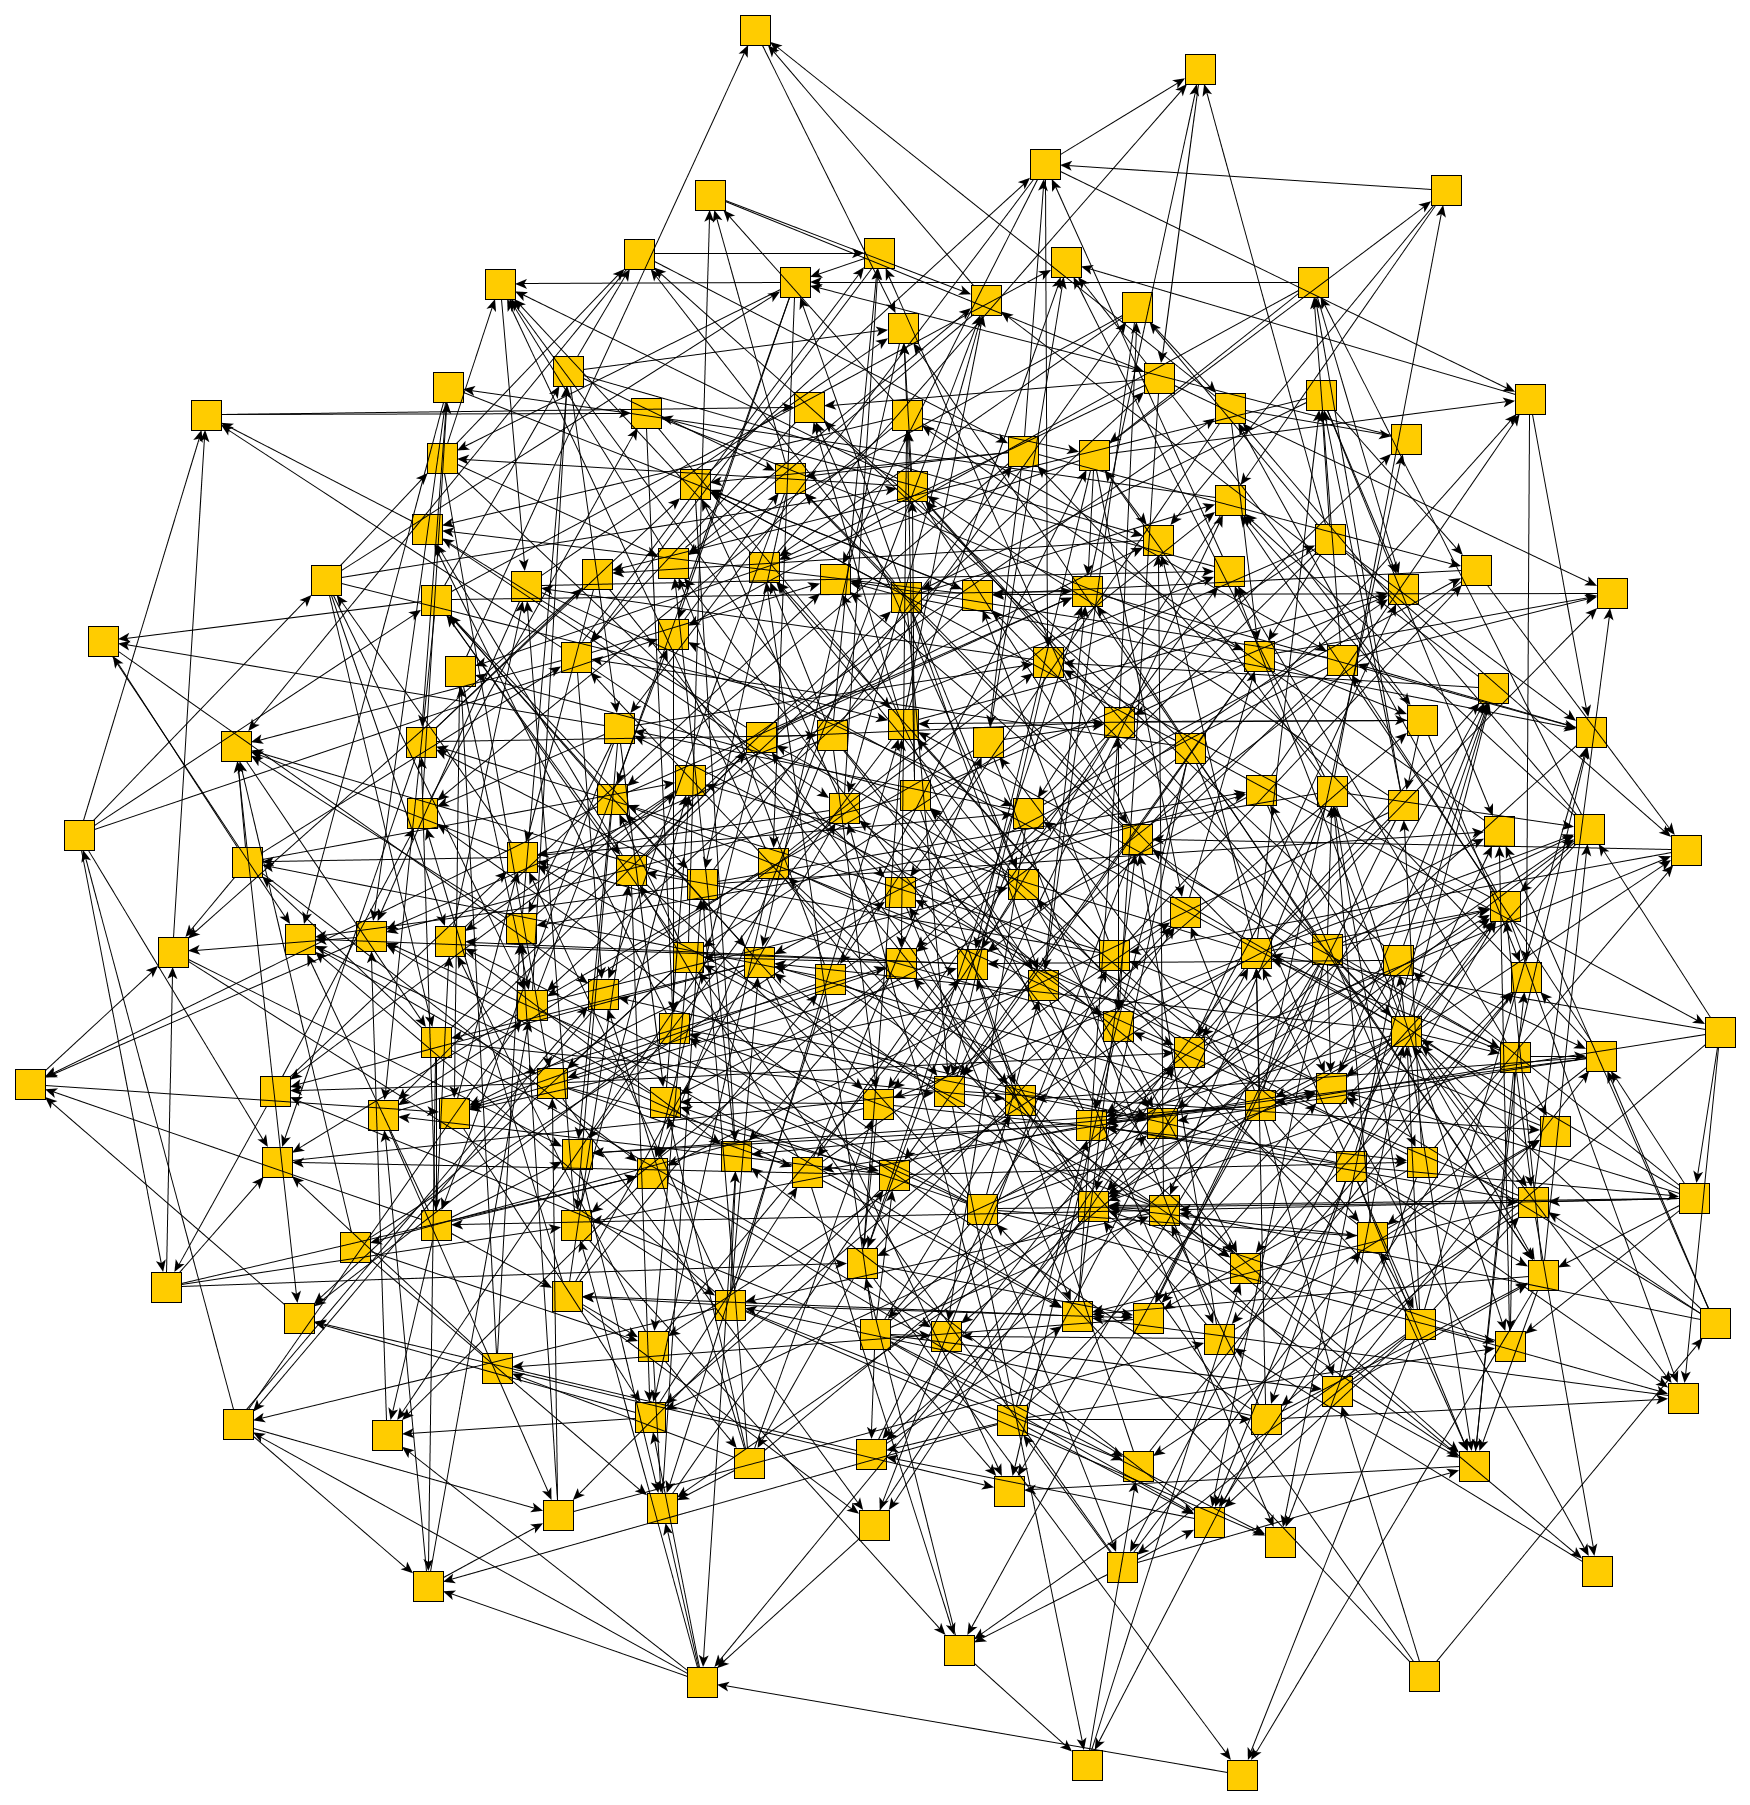
\includegraphics[width=0.9\textwidth]{AFICCMA}
	\caption{Example argumentation framework graph}
\end{figure}

%\begin{subappendices}
%\subchapter{Example sub appendices}
%\end{subappendices}

%\chapter{Second Formal Review Output}
%Insert a copy of the project review form you were given at the end of the review by %the second marker

%\chapter{Diary Sheets (or other project management evidence)}
%Insert diary sheets here together with any project management plan you have

%\chapter{Appendix 4 and following}
%insert content here and for each of the other appendices, the title may be just on a page by itself, the pages of the appendices are not numbered, unless an included document such as a user manual or design document is itself pager numbered.
\end{appendices}

\end{document}
